\chapter{Les plantes sans graines}\label{ch:g4:plants-without-seeds}

Le côté ombragé du vieux mur est tapissé de mousse~; sous les
hêtres, les \omterm{prop:g4:plants-without-seeds:damp}{fougères} déroulent leurs grandes frondes vertes.
Cherche-les tout l'été~: tu n'y trouveras ni \omterm{def:g3:flowers-fruits-seeds:parts}{fleur}, ni \omterm{prop:g3:flowers-fruits-seeds:transform}{fruit}, ni
\omterm{def:g2:from-seed-to-plant:seed}{graine} --- jamais. Et pourtant, \omterm{prop:g4:plants-without-seeds:damp}{mousses} et \omterm{prop:g4:plants-without-seeds:damp}{fougères} se répandent
très bien. Les \omterm{def:g1:plants-around-us:plant}{plantes}, il se trouve, ont plus d'une façon de faire
la génération suivante.

\section{Fougères et mousses~: la reproduction par spores}

\begin{definition}[Spore]\label{def:g4:plants-without-seeds:spore}
Une \emph{spore}\index{spore} est un grain microscopique, fabriqué
en très grand nombre, à partir duquel une nouvelle \omterm{def:g1:plants-around-us:plant}{plante} peut
pousser. Contrairement à une \omterm{def:g2:from-seed-to-plant:seed}{graine}
(\cref{def:g2:from-seed-to-plant:seed}), une spore est un simple
grain \emph{sans \omterm{def:g3:animals-through-seasons:active}{réserve de nourriture} et sans petite \omterm{def:g1:plants-around-us:plant}{plante} toute
prête à l'intérieur} --- c'est un commencement dans le plus simple
appareil.
\end{definition}

\begin{example}[Sous les frondes de la fougère]\label{ex:g4:plants-without-seeds:fern}
Retourne une fronde de fougère à la fin de l'été~: de nettes rangées
de points bruns garnissent son revers. Chaque point est un paquet de
milliers de \omterm{def:g4:plants-without-seeds:spore}{spores}~; à maturité, les paquets s'ouvrent, et les
\omterm{def:g4:plants-without-seeds:spore}{spores} s'envolent au vent comme la plus fine des poussières. Une
\omterm{def:g4:plants-without-seeds:spore}{spore} qui se pose sur un sol humide et ombragé peut devenir --- par
étapes --- une nouvelle fougère.
\end{example}

\begin{omfigure}
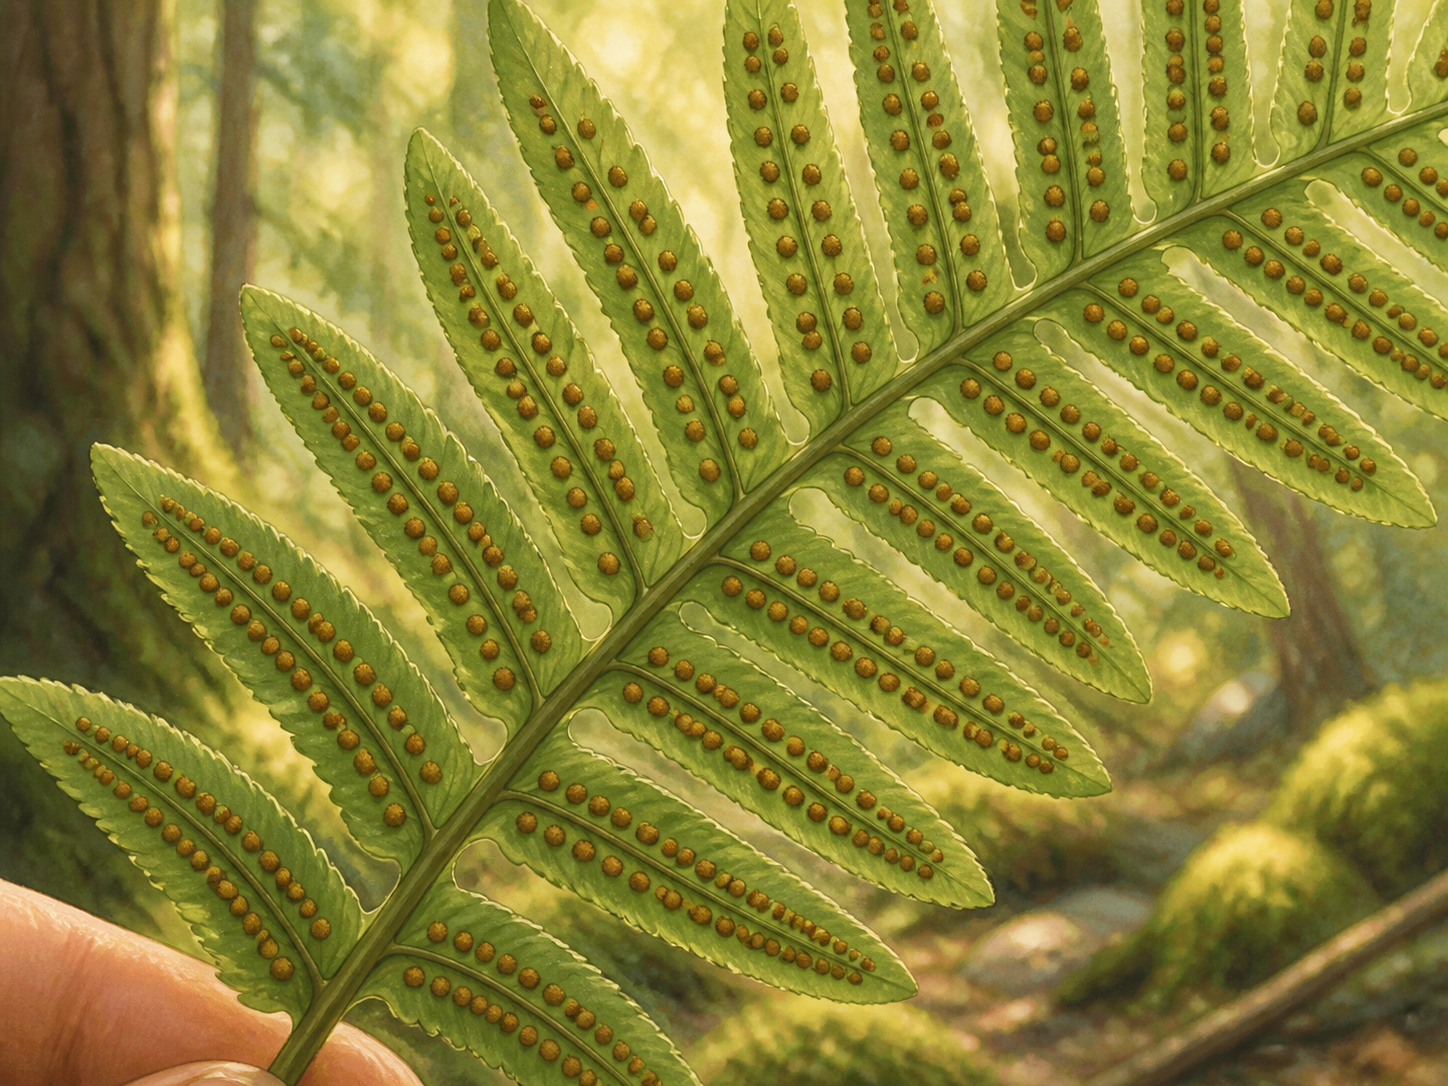
\includegraphics[width=0.56\linewidth]{images/book1/ai/g4-ferns-sori.png}

{\small Sous la fronde~: les nettes rangées de points bruns,
chacun un paquet de milliers de \omterm{def:g4:plants-without-seeds:spore}{spores}.}
\end{omfigure}

\begin{proposition}[Les plantes à spores ont besoin d'humidité]\label{prop:g4:plants-without-seeds:damp}
Les \omterm{def:g1:plants-around-us:plant}{plantes} à \omterm{def:g4:plants-without-seeds:spore}{spores} --- les \emph{mousses}\index{mousse} et les
\emph{fougères}\index{fougère} --- ne peuvent se reproduire que là
où il fait \emph{humide}~: leurs \omterm{def:g4:plants-without-seeds:spore}{spores}, et les stades délicats qui
en sortent, sèchent et meurent dans l'air sec. Voilà pourquoi la
mousse tapisse le mur nord ombragé et jamais le mur sud ensoleillé,
et pourquoi les \omterm{prop:g4:plants-without-seeds:damp}{fougères} se pressent dans les bois humides, sur les
berges et autour des puits.
\end{proposition}
\admitted

\begin{remark}[Une spore n'est pas une graine]\label{rem:g4:plants-without-seeds:sporeseed}
Toutes deux sont des commencements qui voyagent, mais la \omterm{def:g2:from-seed-to-plant:seed}{graine} est
un nécessaire de survie --- enveloppe, réserve, plantule toute prête
--- alors que la \omterm{def:g4:plants-without-seeds:spore}{spore} est nue. D'où les nombres~: les millions de
\omterm{def:g4:plants-without-seeds:spore}{spores} de la fougère contre la douzaine de \omterm{prop:g3:flowers-fruits-seeds:transform}{graines} de la cosse de
haricot. Les commencements nus sont bon marché à fabriquer et
faciles à perdre~; les deux plans font écho à la morue et à
l'éléphante de \cref{prop:g4:animal-reproduction:strategies}.
\end{remark}

\section{De nouvelles plantes sans le moindre semis}

\begin{definition}[Reproduction végétative]\label{def:g4:plants-without-seeds:vegetative}
Beaucoup de \omterm{def:g1:plants-around-us:plant}{plantes} savent aussi faire de nouvelles \omterm{def:g1:plants-around-us:plant}{plantes}
\emph{directement à partir d'un morceau d'elles-mêmes} --- sans
\omterm{def:g4:plants-without-seeds:spore}{spores}, sans \omterm{prop:g3:flowers-fruits-seeds:transform}{graines}, avec un seul parent. C'est la \emph{reproduction
végétative}\index{reproduction végétative}. La nouvelle \omterm{def:g1:plants-around-us:plant}{plante} est
une continuation vivante de l'ancienne, et lui ressemble exactement.
\end{definition}

\begin{example}[Les stolons du fraisier]\label{ex:g4:plants-without-seeds:runner}
Un fraisier envoie sur le sol de longues \omterm{def:g1:plants-around-us:parts}{tiges} horizontales et fines
--- les \emph{stolons}\index{stolon}. Là où un stolon touche terre,
il s'enracine, pousse des \omterm{def:g1:plants-around-us:parts}{feuilles} et devient un fraisier complet~;
le stolon se dessèche ensuite, et l'enfant se tient seul. Une \omterm{def:g1:plants-around-us:plant}{plante}
devient un carré entier sans qu'une seule \omterm{def:g2:from-seed-to-plant:seed}{graine} ait été semée.
\end{example}

\begin{example}[Bulbes et tubercules]\label{ex:g4:plants-without-seeds:bulbtuber}
Le \emph{bulbe}\index{bulbe} de tulipe et le
\emph{tubercule}\index{tubercule} de pomme de terre sont des
réserves souterraines --- et des nécessaires de départ. Laissé en
terre, un \omterm{ex:g4:plants-without-seeds:bulbtuber}{bulbe} se divise en bulbes-filles, chacun une future
tulipe~; chaque «~\omterm{def:g1:the-five-senses:sense}{œil}~» d'une pomme de terre qui germe peut donner
une \omterm{def:g1:plants-around-us:plant}{plante} entière. Les jardiniers plantent des pommes de terre, pas
des \omterm{prop:g3:flowers-fruits-seeds:transform}{graines} de pomme de terre.
\end{example}

\begin{method}[Faire une bouture]\label{met:g4:plants-without-seeds:cutting}
Les jardiniers imitent la \omterm{def:g4:plants-without-seeds:vegetative}{reproduction végétative} avec des
\emph{boutures}\index{bouture}~:
\begin{enumerate}
  \item coupe une \omterm{prop:g2:from-seed-to-plant:cycle}{jeune pousse} saine, longue comme la main, sur la
        \omterm{def:g1:plants-around-us:plant}{plante} mère (la menthe, le saule et les géraniums
        s'y prêtent bien)~;
  \item enlève les \omterm{def:g1:plants-around-us:parts}{feuilles} du bas et mets la pousse dans l'eau ou
        dans une terre humide~;
  \item attends~: en quelques jours ou quelques semaines, des
        \omterm{def:g1:plants-around-us:parts}{racines} poussent sur la \omterm{def:g1:plants-around-us:parts}{tige} coupée~;
  \item plante-la --- une nouvelle \omterm{def:g1:plants-around-us:plant}{plante} complète, identique à son
        unique parent.
\end{enumerate}
\end{method}

\begin{remark}[Un seul parent, des copies exactes]\label{rem:g4:plants-without-seeds:copy}
Les \omterm{prop:g3:flowers-fruits-seeds:transform}{graines} mélangent deux parents
(\cref{rem:g4:animal-reproduction:mix} vaut aussi pour les \omterm{def:g1:plants-around-us:plant}{plantes},
par le \omterm{def:g3:flowers-fruits-seeds:parts}{pollen})~; la \omterm{def:g4:plants-without-seeds:vegetative}{reproduction végétative} en recopie un seul. Voilà
pourquoi chaque arbre d'une variété de pomme nommée est obtenu par
bouture ou par greffe, jamais à partir de pépins~: le verger veut
des copies exactes d'un excellent arbre. Le prix de la copie est
l'uniformité --- un verger d'arbres identiques partage des
faiblesses identiques, comme une année ultérieure le montrera.
\end{remark}

\section{Exercices}

\begin{exercise}[$\star$]\label{exo:g4:plants-without-seeds:1}
Nomme deux \omterm{def:g1:plants-around-us:plant}{plantes} qui ne font jamais de \omterm{prop:g3:flowers-fruits-seeds:transform}{graines}. Comment se
reproduisent-elles~?
\end{exercise}

\begin{exercise}[$\star$]\label{exo:g4:plants-without-seeds:2}
Donne deux différences entre une \omterm{def:g4:plants-without-seeds:spore}{spore} et une \omterm{def:g2:from-seed-to-plant:seed}{graine}.
\end{exercise}

\begin{exercise}[$\star$]\label{exo:g4:plants-without-seeds:3}
Où sont fabriquées les \omterm{def:g4:plants-without-seeds:spore}{spores} de la fougère~? Décris ce que tu
trouves sous une fronde à la fin de l'été.
\end{exercise}

\begin{exercise}[$\star$]\label{exo:g4:plants-without-seeds:4}
Pourquoi la mousse pousse-t-elle sur le mur nord ombragé et pas sur
le mur sud ensoleillé~?
\end{exercise}

\begin{exercise}[$\star$]\label{exo:g4:plants-without-seeds:5}
Qu'est-ce que la \omterm{def:g4:plants-without-seeds:vegetative}{reproduction végétative}~? Combien de parents
demande-t-elle~?
\end{exercise}

\begin{exercise}[$\star$]\label{exo:g4:plants-without-seeds:6}
Raconte l'histoire d'un stolon de fraisier, de la première \omterm{def:g1:plants-around-us:parts}{tige} à
l'enfant qui se tient seul.
\end{exercise}

\begin{exercise}[$\star$]\label{exo:g4:plants-without-seeds:7}
Pourquoi les jardiniers plantent-ils des pommes de terre plutôt que
de semer des \omterm{prop:g3:flowers-fruits-seeds:transform}{graines} de pomme de terre~? Que peut faire chaque
«~\omterm{def:g1:the-five-senses:sense}{œil}~»~?
\end{exercise}

\begin{exercise}[$\star$]\label{exo:g4:plants-without-seeds:8}
À toi d'essayer~: prends une bouture de menthe selon
\cref{met:g4:plants-without-seeds:cutting} et mets-la dans un verre
d'eau sur le rebord de la fenêtre. Qu'apparaît-il, et au bout de
combien de temps environ~?
\end{exercise}

\begin{exercise}[$\star\star$]\label{exo:g4:plants-without-seeds:9}
La fougère fait des millions de \omterm{def:g4:plants-without-seeds:spore}{spores}~; la cosse de haricot, une
douzaine de \omterm{prop:g3:flowers-fruits-seeds:transform}{graines}. Explique la différence de nombre avec
\cref{rem:g4:plants-without-seeds:sporeseed} --- et nomme le couple
d'\omterm{def:g1:animals-around-us:animal}{animaux} dont elles reprennent les stratégies.
\end{exercise}

\begin{exercise}[$\star\star$]\label{exo:g4:plants-without-seeds:10}
Une jardinière trouve les nouveaux fraisiers identiques au pied
mère, alors que ses haricots varient un peu par rapport à leurs
parents. Explique les deux observations avec
\cref{rem:g4:plants-without-seeds:copy}.
\end{exercise}

\begin{exercise}[$\star\star\star$]\label{exo:g4:plants-without-seeds:11}
Une \omterm{def:g1:plants-around-us:tree}{branche} de saule arrachée par une crue d'hiver, emportée par le
courant et échouée sur un banc de vase, devient souvent un nouveau
saule. De quelle sorte de reproduction s'agit-il --- et pourquoi les
rivières sont-elles si souvent bordées de saules~? Qu'a fait la crue
que la jardinière de
\cref{met:g4:plants-without-seeds:cutting} fait avec un sécateur~?
\end{exercise}
